\chapter{Approximation Method Performance}

In theory, the $\varepsilon-$complexity of a continuous function is found using the minimum error over a possibly infinite set of approximation methods. To be computationally efficient, this set of approximation methods needs to be finite and in practice, is restricted to some relatively small set of approximation methods. The initial implementation of the $\varepsilon-$complexity algorithm used piece-wise polynomial interpolation. Our implementation extends the number of methods used to three: basis splines(B-splines) of up to order 4, 
cubic splines and the interpolating subdivision we refer to as the lifting scheme after Sweldens \cite{sweldens1998}. 

The goal in including more approximation methods was to test whether drawing on a richer set of functions would improve the performance of the $\varepsilon-$complexity coefficients. In this chapter, we gauge the approximation methods in two ways. First, we measure the average approximation error of each method on a range of functions. 
Secondly, we test the 
ability of the complexity coefficients to discriminate between two sets of closely related time series. Based on these experiments, increasing the accuracy of the approximation did not lead to better performance in the discrimination task. In fact, the cubic spline method which was less accurate in terms of approximation errors performed as well or better than the more accurate B-spline method.

A separate concern was the computational efficiency of the approximation methods. Computational efficiency becomes a pressing issue as the size of a data set increases. The EEG time series studied in the next Chapter 5 were moderately sized by modern standards, consisting of several million points per time series. But even at this size computational efficiency became an issue when using the less efficient B-spline algorithm. The B-spline method, although the most accurate approximation method of the three tested, uses matrix operations which are at least quadratic both in space and time efficiency. Based on both computational efficiency and classification performance we have used the cubic spline method as our default for computing the complexity coefficients in our \texttt{R} implementation of the algorithm and in our applied work in the following two chapters.

\section{Simulations Tests}

For these experiments, we used six simulations methods comprised of both deterministic and random processes. We have presented all but one of these functions in the background section. The \textit{logisitc map}  is a single parameter nonlinear deterministic discrete difference equation defined
\[
  x_t = r(x_{t-1})(1 - x_{t-1}).
\]
For values of $r$ close to but less than 4 the logistic map exhibits chaotic behavior and the graph of the function
changes significantly for small perturbations of the $r$ parameter. The other simulations used were the ARMA and FARIMA processes, the random-phase Weierstrass function, fractional Brownian motion (FBM) and the Cauchy process. 

Two sets of models were created with each set having slightly varying initial parameters. For each simulation, the initial parameters perturbed by selecting a parameter uniformly in a window about the initial parameter value. A sample from each simulation group is shown in \ref{fig:jitter-ts}. 

\begin{figure}[!htbp]
  \begin{center}
  % \begin{picture}(60,60)
  % ./figs/coeff-interp-simple-functions1.pdf
  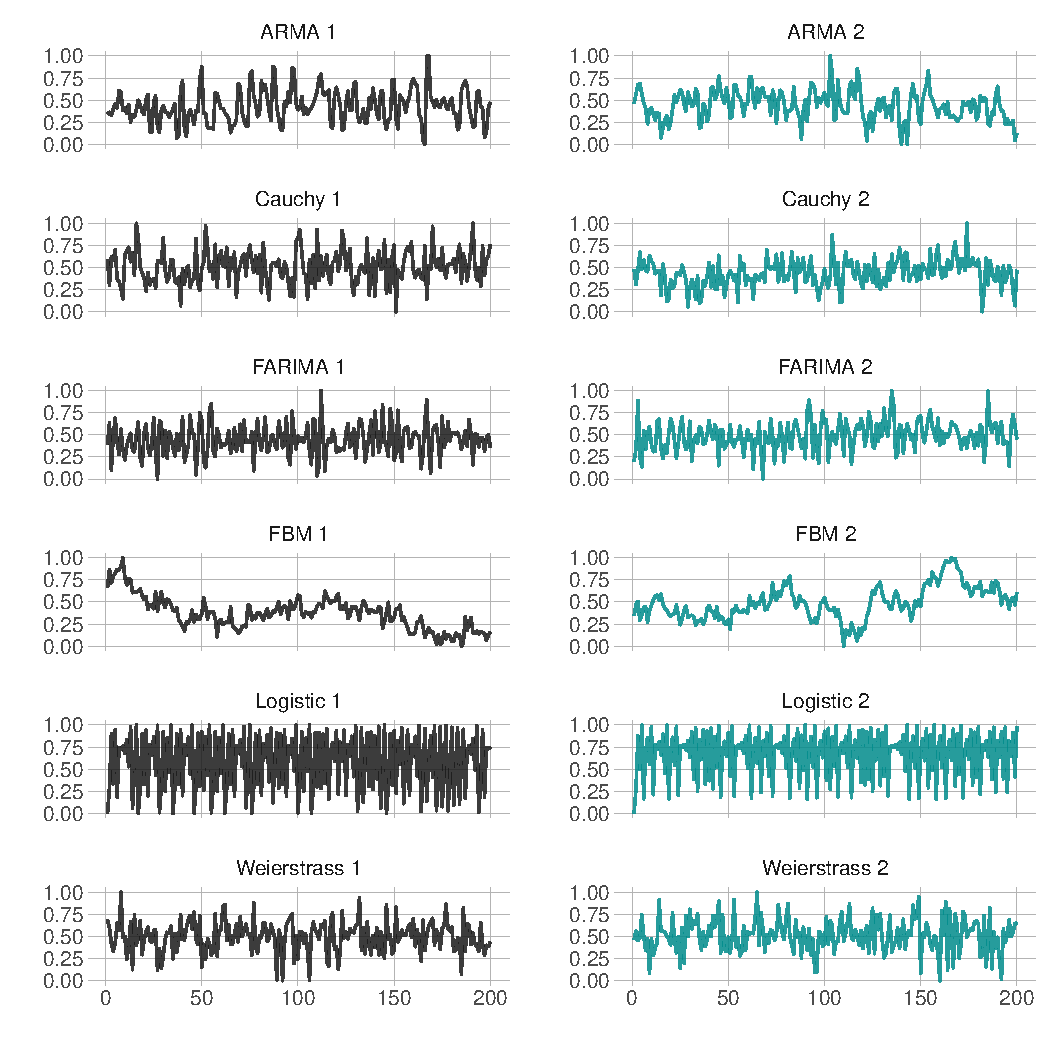
\includegraphics[width = \textwidth, keepaspectratio]{./figs/sim_jitter_plot_jitter_timeseries.pdf}
  % \end{picture}
  \end{center} 
  \caption{Sample functions from each simulation group.  }
   \label{fig:jitter-ts}
\end{figure}


% The approximation methods accuracy was compared based on the mean squared error(MSE) of the approximation and secondly the classification accuracy when the complexity coefficients computed by each method were used to classify each simulation. 
In addition to the three individual approximation methods -- cubic splines, B-splines, and the lifting method -- for a fourth method the approximation error was calculated as the minimum error over all methods. Shown in \ref{fig:lift-lm} is an example of log-log linear fit of the approximation errors against the sample fraction for a single function from each simulation type. For this figure, the lifting method was used. The figure is a simple diagnostic check that the log-log fit was roughly linear and the results of the test were similar to that shown in \ref{fig:lift-lm} for each approximation method. 


\begin{figure}[!htbp]
  \begin{center}
  % \begin{picture}(60,60)
  % ./figs/coeff-interp-simple-functions1.pdf
  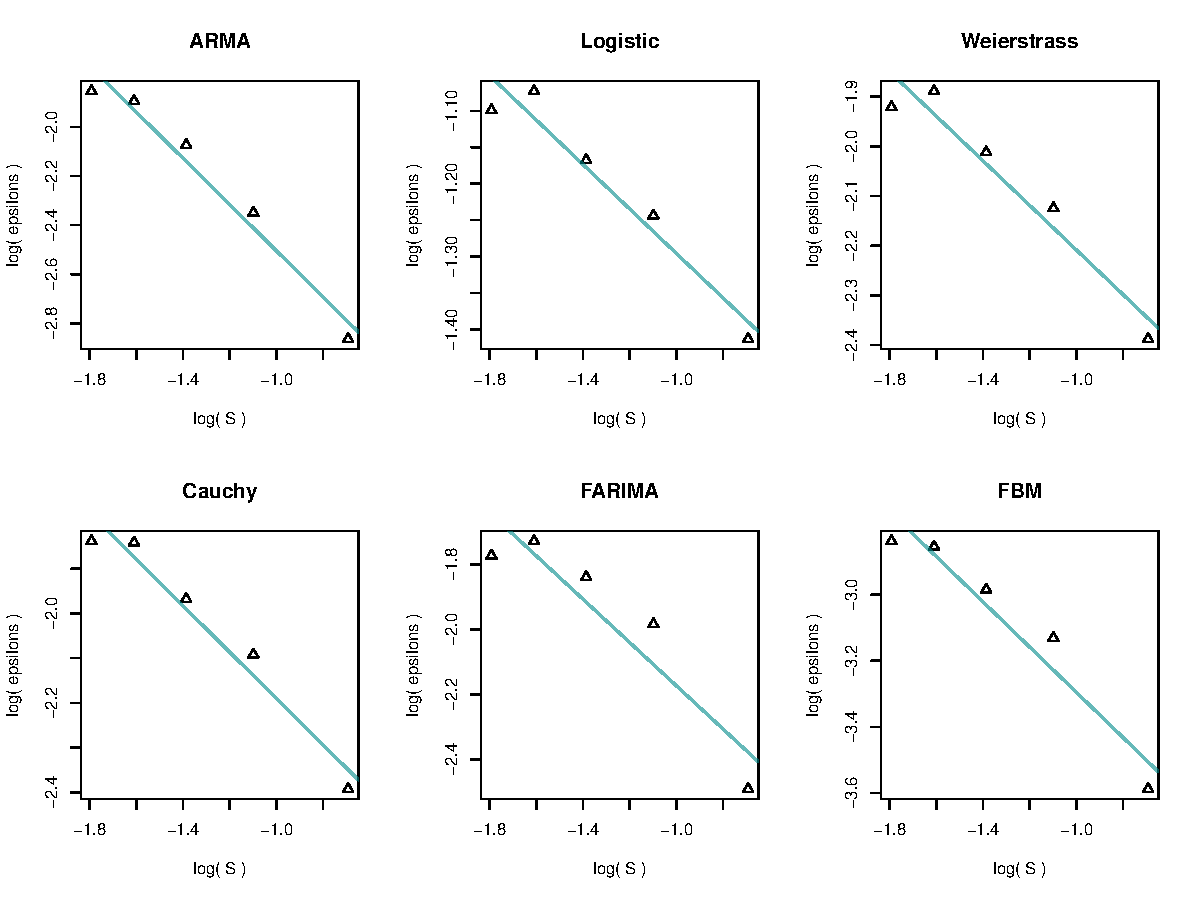
\includegraphics[width = \textwidth, keepaspectratio]{./figs/sim_jitter_plot-sim-fits.pdf}
  % \end{picture}
  \end{center} 
  \caption{Least squares fits used to compute the complexity 
  coefficients using the lifting scheme.}
  \label{fig:lift-lm}
\end{figure}


Figure \ref{fig:feature-space} is a scatterplot of the complexity coefficients generated by each approximation method for the two groups of simulations. Each point represents where an individual function lies in the feature space of the two complexity coefficients $A$ and $B$. The coefficient values have been normalized to the $[0,1]$ interval show the plots only show the relative distribution of the functions. Although it is hard to distinguish the denser regions, the plot shows that the complexity coefficients are distributed
similarly for each method -- the complexity coefficients for a given simulation lie in the same region of the function space for each method. Several functions are also linearly separable in coefficient space -- a line could easily be drawn that divides the two groups. For example, the samples of the logistic function are tightly grouped in the upper right and corner and fractional Brownian motion and the ARMA process are also well separated in the lower left-hand corner. The separability of the two groups is quantified in by the classification error in Table \ref{tab:error-all} which we discuss in more detail below.

\begin{figure}[!htbp]
  \begin{center}
  % \begin{picture}(60,60)
  % ./figs/coeff-interp-simple-functions1.pdf
  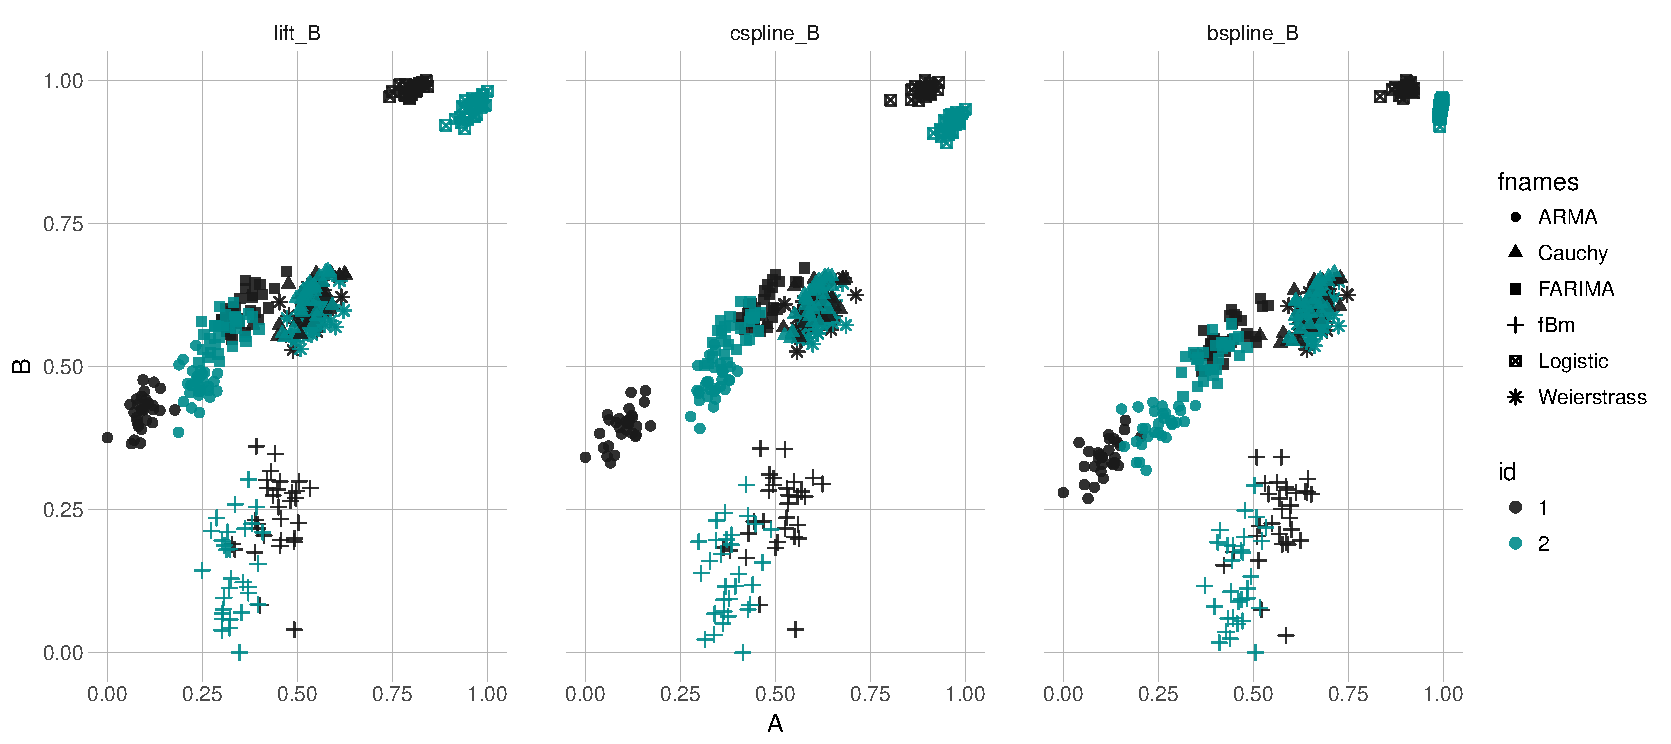
\includegraphics[width = \textwidth, keepaspectratio]{./figs/ecomplex_approx-feature-space.pdf}
  % \end{picture}
  \end{center}
  \caption{Functions from the two simulation groups plotted in the 
  complexity coefficient space.}
  \label{fig:feature-space} 
\end{figure}

We finally observe in Figure \ref{fig:feature-space} the direction in which, when possible, the functions can be linearly separated.
 In the following chapter, we compare how the complexity coefficients and fractal dimension vary with the parameters several functions. 
 Based on those tests it is unclear whether the intercept coefficient $A$ adds contributes information that can be used in discriminating two functions that are not found in slope coefficient $B$.
 % and the variogram estimator of fractal dimension were reflected changes in the parameters controlling the H\"older class of the function. 
 % Except in the case of the random phase Weierstrass function, the intercept coefficient $A$ seemed to follow a similar pattern as the slope coefficient. 
 However, in the figure \ref{fig:feature-space} for the function types that are readily separable -- FBM and the ARMA and logistic simulations --  both the slope and intercept coefficient appear to be useful in separating the two sets of simulations. For example, both the FBM and ARMA simulations are well separated along the $A$-axis. Although how best to interpret each of the coefficients is not clear, both appear useful for separating related functions.

Using the two sets of simulations described above, with 30 samples taken from each parameter group, the approximation error and classification accuracy of each approximation method was tested. 
Tables \ref{tab:epsilons-all} and \ref{tab:error-all} show the mean approximation error for each method and the overall classification accuracy when using only the two complexity coefficients as predictors. The B-spline approximation had the lowest MSE approximation for all functions
and the combined method simply reflects the B-spline errors. 
The lift approximation method also has slightly lower
MSE for most functions. 


\begin{table}[!htbp] \centering 
\begin{tabular}{@{\extracolsep{1pt}} ccccccc} 
\\[-1.8ex]\hline 
\hline \\[-1.8ex] 
  Function & Lift & Cspline & Bspline & Combined \\ \hline 
ARMA       & 0.10  & 0.11    & 0.07 & 0.07 \\ 
Cauchy       & 0.09  & 0.10  & 0.06 & 0.06 \\ 
FARIMA       & 0.13  & 0.14  & 0.08 & 0.08 \\ 
FBM          & 0.03  & 0.04  & 0.02 & 0.02 \\ 
Logistic     & 0.30  & 0.32  & 0.20 & 0.20 \\ 
Weierstrass  & 0.14  & 0.15  & 0.09 & 0.09 \\ 
\hline \\[-1.8ex] 
          \end{tabular} 
  \caption{Mean of the approximation errors of each method 
         summed over each downsampling level. 
           Errors were computed on 30 simulations of each model. 
             }
  \label{tab:epsilons-all}
\end{table}



\begin{table}[!htbp] \centering 
\begin{tabular}{@{\extracolsep{1pt}} ccccccc} 
\\[-1.8ex]\hline 
\hline \\[-1.8ex] 
Function    &  Lift & Cspline & Bpsline  & Combined 
                                       \\ \hline
ARMA        & 0.03 &   0.00 &   0.07 &   0.07  \\ 
Cauchy      & 0.65 &   0.53 &   0.52  &    0.53  \\ 
FARIMA      & 0.32 &   0.30 &   0.32  &    0.33 \\ 
FBM         & 0.20  &   0.22  & 0.20 &  0.22  \\ 
Logistic    & 0.00 &   0.00 &   0.00  &    0.02  \\ 
Weierstrass & 0.50 &   0.43 &   0.45  &    0.45  \\
\hline \\[-1.8ex] 
          \end{tabular} 
  \caption{Classification errors using complexity coefficients  
  $A$ and $B$ for each approximation method using a random 
  forest classifier.}
  \label{tab:error-all}
\end{table}

The complexity coefficients as computed by each approximation method were used to classify the two
sets of simulations. A random forest classifier was used and the overall out-of-bag classification error is shown in \ref{tab:error-all}. No method is dominant for all simulation types, and the cubic spline method performs as well or better than the two approximation methods. 

Based only on the previous two tests there is 
not a clear reason to choose 
one of the approximation methods over another. Classification performance did not seem affected by the slightly lower approximation accuracy of the lifting and cubic spline methods. However, both the cubic spline and lifting approximation methods are computationally more efficient. Both methods are computationally linear in the number of inputs, or $O(n)$, and both are linear or constant in terms of their space complexity -- the amount of memory needed to store intermediate computations is a linear or constant function of the size of the inputs. 
Figure \ref{fig:benchmark} show the computational time of 
each method as a function of the $\log$ of the input size.

\section{Computational Complexity}

For our implementation, we scaled the number of basis elements used in the B-spline method with the number of data points. Growing the number of basis elements with the size of the input made the B-spline method infeasible for time series over a few thousand points in length. Although both 
the lifting method and cubic splines are linear, our lifting 
implementation was written entirely in the \texttt{R} 
language while the most of the computations in the cubic spline method are written in the more computationally efficient \texttt{C} language. 

\begin{figure}[!htbp]
  \begin{center}
  % \begin{picture}(60,60)
  % ./figs/coeff-interp-simple-functions1.pdf
  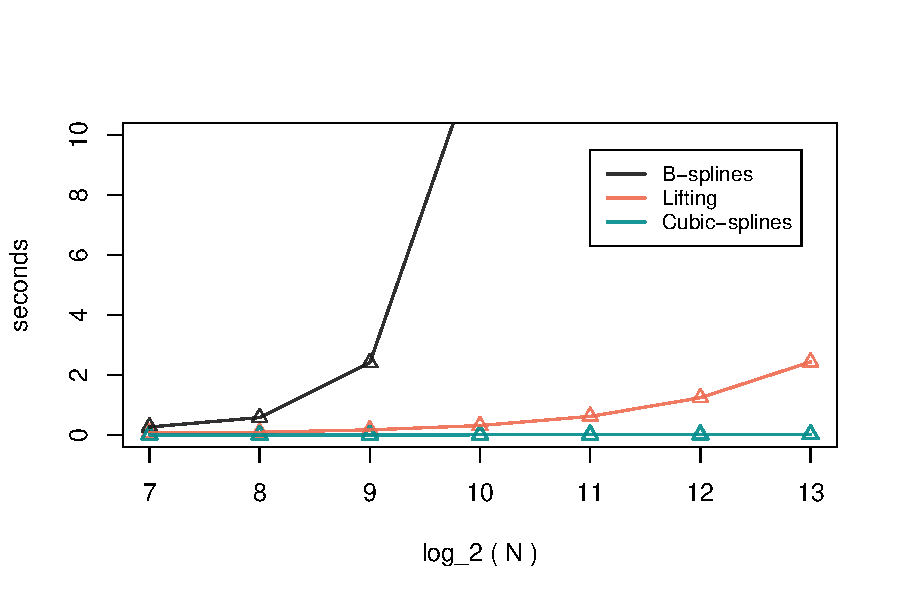
\includegraphics[width = \textwidth, keepaspectratio]{./figs/benchmark-benchmark.pdf}
  % \end{picture}
  \end{center}
  \caption{Computational time in seconds as function of 
  the $\log$ of the inputs.}
  \label{fig:benchmark} 
\end{figure}

Finally, we tested whether the classification error varied with the loss function used to compute approximation error. Again, accuracy computed as the out-of-bag classification accuracy of a random forest classifier. Both the mean squared error, mean absolute error(MAE) loss function performed similarly with MSE performing slightly better. 


The purpose of the preceding test was to verify that the approximation methods used in our implementation of the $\varepsilon-$complexity algorithm behaved as expected and to compare the performance of the complexity coefficients as the algorithm parameters where altered. Based on these tests we used cubic splines as the approximation method and set MSE as our loss function for the application to EEG classification discussed in chapter 5.


\begin{table}[!htbp] \centering 
\begin{tabular}{@{\extracolsep{1pt}} ccccccc} 
\\[-1.8ex]\hline 
\hline \\[-1.8ex] 
Function          &    MAE  & Max  & MSE \\
\hline \\[-1.8ex]  
ARMA         &   0.00  & 0.33 &  0.03  \\ 
Cauchy       &   0.52  & 0.47 &  0.66  \\ 
FARIMA       &   0.18  & 0.39 &  0.22  \\ 
FBM          &   0.13  & 0.33 &  0.16  \\ 
Logistic     &   0.01  & 0.18 &  0.00  \\ 
Weierstrass  &   0.44  & 0.51 &  0.53  \\
\hline \\[-1.8ex] 
          \end{tabular}  
  \caption{Classification error using a random forest classifier 
           and three different loss functions.}
  \label{tab:error-mse}
\end{table}

% Since both complexity coefficients were useful 
% in discriminating between functions drawn from similar sets of parameters, we also used both coefficients to 




